\mychapter{2}{Introduction}
%
% Problems and objectives of your research should be clearly stated and placed in the context of a broader field. An extensive bibliography should be included. This section should lead the reader to each question or hypothesis that you’re testing in each aim. Significance of the project should be also included here.
%
During sleep, animals lose awareness of the environment as well as their will to affect it, but this cost of losing of touch is accompanied by a provisional guarantee on the stability of the body: by drastically limiting its interaction with the environment, the body can refocus its energy on other needs, such as growth, cleanup, and repair. The value of this process might be appreciated in terms of the consequences of sleep deprivation - a long list including, loss of sex drive, weakened immunity, increased blood pressure, memory impairment, and increased risk for many diseases like Alzheimer's dementia (AD). So while unconsciousness is the most obvious feature of sleep, it is just a side-effect of this profound state change which facilitates critical homeostatic processes throughout the body - especially in the brain. Around sleep onset, movement, sensation, and cognition are reduced along with the metabolic demand in tissues serving these functions, thus permitting respiration to slow and the heart relax. As the brain falls deeper into sleep, the concentration of neuromodulatory transmitters, like norepinephrine and serotonin, decrease, and neuronal activity increasingly alternates between active and inactive firing states modulated by $\sim$1 Hz waveforms called slow waves (SW). In parallel, glia, especially astrocytes, undergo a major shift in activity; for example, altering ionic composition and permitting greater flow of interstitial fluid, reducing their rate of lactate production, and increasing phagocytosis of fatigued neural components. Determining how the function and dysfunction of these processes promote and reduce brain health will improve our basic understanding of sleep and may introduce new therapeutic targets. With my dissertation, I hope to contribute to the science of human slow wave sleep by identifying patterns of macroscopic electrophysiology that support memory consolidation and by imaging glymphatic activity to evaluate its role in aging and dementia. Below, I begin with a broad survey of the literature relevant to slow wave sleep and its relationship to memory, aging, and dementia.
%!!!%

%%%%%%%%%%%%%%%%%%%%%%%%%%%%%%%%%%%%%%%%%%%%%%%%%%%%%%%%%%%%%%%%%%%%%%%%%%%%%%%%%%%%
%%%%%%%%%%%%%%%%%%%%%%%%%%%%%%%%%%%%%%%%%%%%%%%%%%%%%%%%%%%%%%%%%%%%%%%%%%%%%%%%%%%%
\section*{Sleep staging}
%%%%%%%%%%%%%%%%%%%%%%%%%%%%%%%%%%%%%%%%%%%%%%%%%%%%%%%%%%%%%%%%%%%%%%%%%%%%%%%%%%%%
%%%%%%%%%%%%%%%%%%%%%%%%%%%%%%%%%%%%%%%%%%%%%%%%%%%%%%%%%%%%%%%%%%%%%%%%%%%%%%%%%%%%
Sleep stages were defined by Allan Rechtschaffen and Anthony Kales in 1968 based on a method of evaluating polysomnography (PSG) comprised of three types of recordings: (1) electroencephalogram (EEG) derived from at least two electrodes placed near the center of the scalp to measure brain activity, (2) electrooculogram (EOG) ideally placed above and below the eyes to measure eye movements, (3) electromusculogram (EMG) ideally placed on and beneath the chin to measure general muscle tone \citep{Kales1968}. These three signals are then visually evaluated to stage sleep in 30 second epochs roughly according to the descriptions below:
\begin{enumerate}
\item[] Stage 1: Non-REM stage 1, abbreviated as NREM1, is a transitory stage of sleep onset and might be characterized as a drowsy restfulness. During this period eye movement slows and muscle tone begins to decrease. Also during this stage, the 8-12Hz alpha rhythm usually present when an awake subject closes their eyes begins to disappear; however, brief bursts of a slightly higher frequency around 12-14 Hz, but with lower voltage, called spindles, may be evident.
\item[] Stages 2-4: NREM2-4 are increasing depths of sleep. Starting with NREM2, the most prominent feature of sleep, the slow wave (SW), begins to emerge and persist through NREM4, which is why these three stages are collectively referred to as slow wave sleep (SWS). The incidence of SWs per 30 sec epoch defines the depth of sleep with thresholds of $<20\%$, $20-50\%$, $>50\%$ defining NREM2-4, respectively. Additionally, during NREM2 and 3, spindles (12-14 Hz at least .5 sec in duration) may be present.
\item[] Stage 5: Rapid eye movement, or REM sleep, has also been called paradoxical sleep because it significantly deviates from the EEG patterns observed during NREM, and rather appears with low-voltage mixed-frequency signals very similar to a waking EEG. However, this paradoxical activity can be distinguished with the rest of the PSG since muscle tone remains low, but eye movement becomes rapid.
%\item[] Stage 6: Wake, finally, is distinguished with a high muscle tone, moderate eye movement, and a low-voltage mixed frequency signal, possibly including alpha oscillations.
\end{enumerate}
In addition to these five sleep stages, are criteria for marking epochs during wake, movements, or obscured by too many artifacts to properly score.

%%%%%%%%%%%%%%%%%%%%%%%%%%%%%%%%%%%%%%%%%%%%%%%%%%%%%%%%%%%%%%%%%%%%%%%%%%%%%%%%%%
%%%%%%%%%%%%%%%%%%%%%%%%%%%%%%%%%%%%%%%%%%%%%%%%%%%%%%%%%%%%%%%%%%%%%%%%%%%%%%%%%%
\section*{The slow wave}
%%%%%%%%%%%%%%%%%%%%%%%%%%%%%%%%%%%%%%%%%%%%%%%%%%%%%%%%%%%%%%%%%%%%%%%%%%%%%%%%%%
%%%%%%%%%%%%%%%%%%%%%%%%%%%%%%%%%%%%%%%%%%%%%%%%%%%%%%%%%%%%%%%%%%%%%%%%%%%%%%%%%%
The namesake for slow wave sleep is naturally its most distinctive feature. Although this waveform is well-studied, there is still uncertainty about how to define it, which brain regions generate it, and the mechanisms that give rise to it. 

%%%%%%%%%%%%%%%%%%%%%%%%%%%%%%%%%%%%%%%%%%%%%%%%%%%%%%%%%%%%%%%%%%%%%%%%%%%%%%%%%%%%
\subsection{Slow waves and oscillations}
%%%%%%%%%%%%%%%%%%%%%%%%%%%%%%%%%%%%%%%%%%%%%%%%%%%%%%%%%%%%%%%%%%%%%%%%%%%%%%%%%%%%
This waveform was initially defined by R$\&$K to be between .5-2 Hz, but it also common to define the band as $<1$, $.1-1$, or $1-4$ Hz, and further complicating the terminology are the additional distinctions of delta waves, infraslow waves, and slow oscillations \citep{Amzica1995a, Vyazovskiy2013,Crunelli2010, Crunelli2018}. The SW was first observed in scalp EEG and interpreted as globally synchronized brain activity, but in 1993, a series of papers by Steriade and colleagues demonstrated that neuronal membrane potentials were modulated at a low frequencies with depolarizing/hyperpolarizing phases, which they defined as $<1$ Hz and called a slow oscillation (SO), and coincident with low frequency waveforms in the field potentials \citep{Steriade1993,Steriade1993a,Steriade1993b}. It is worth noting that the frequency range for the SO defined by Steriade is enormous, covering any periodic activity lasting longer than 1 sec, but while dubious, is still frequently used. This unfortunate because recent research efforts have identified activity $<.1$ Hz, to be distinct from the SO \citep{Mitra2014, Schwalm2017, Lecci2017,Piantoni2017}; in contrast, delta waves, typically defined as 1-4 Hz, seem to be closely related, and perhaps even arising from the same mechanisms as .1-1 Hz activity \citep{Crunelli2018}. SWs during sleep, regardless of band, were generally considered to be global phenomena, until the new millenium $-$ although there were some earlier suggestions \citep{Mukhametov1977,WERTH1997,Finelli2001}. The view that SWs instead tend to occur locally was solidified with early intracranial studies \citep{Cash2009,Nir2011}. The more rare global SW were more likely to begin frontally and later be detected in parietal then temporal lobes. Intracranial work was also able to replicate the SO finding in humans \citep{Cash2009}. Today, this SW modulation of neuronal firing rates is more commonly referred to as UP and DOWN states\citep{Sanchez-Vives2000, Cash2009}. For clarity and brevity, I will use SW to refer to modulations in field potential, and SO to refer to modulations of neuronal excitability at the same frequency as SO.

%%%%%%%%%%%%%%%%%%%%%%%%%%%%%%%%%%%%%%%%%%%%%%%%%%%%%%%%%%%%%%%%%%%%%%%%%%%%%%%%%%%%
\subsection*{Cortico-thalamic interaction}
%%%%%%%%%%%%%%%%%%%%%%%%%%%%%%%%%%%%%%%%%%%%%%%%%%%%%%%%%%%%%%%%%%%%%%%%%%%%%%%%%%%%
The seminal papers from Steriade et. al. also established that reticular thalamic and cortically projecting thalamic neurons exhibit SOs, but the extent to which the thalamus is involved in the generation of this activity has been a matter of contention ever since \citep{Steriade1993b, Crunelli2010, Crunelli2018}. Because SO continue to be observed in brain preparations with lesions to or removal of the thalamus, the cortex has been generally considered to be the primary generator of SOs \citep{Steriade1993b, Timofeev1996}. Although, there is evidence that the isolated thalamus can also generate SOs, it seems that this activity depends on mGluR1 stimulation, which is mediated by cortical neurons \textit{in vivo}, so the emerging view is that while the thalamus can produce these waves, it probably plays a more auxiliary role supporting SW/SO which are generated cortically \citep{Blethyn2006a, Crunelli2010, Mak-Mccully2017}.

%%%%%%%%%%%%%%%%%%%%%%%%%%%%%%%%%%%%%%%%%%%%%%%%%%%%%%%%%%%%%%%%%%%%%%%%%%%%%%%%%%%%
\subsection*{Cellular mechanisms}
%%%%%%%%%%%%%%%%%%%%%%%%%%%%%%%%%%%%%%%%%%%%%%%%%%%%%%%%%%%%%%%%%%%%%%%%%%%%%%%%%%%%
In the cortex, hyperpolarized down-states seem to be due to a combination of afterhyperpolarizations produced by Ca$^{2+}$ mediated K$^+$ currents as well as disfacilitation, i.e. processes reducing excitation \citep{Timofeev2001, Buzsaki2012, Mak-Mccully2017}. In contrast, thalamic SO depend pacemaker low-threshold spiking (LTS) and involve an interplay of currents including K$^+$ leak, I$_T$, I$_{CAN}$, and I$_h$  \citep{Hughes2002,Blethyn2006a, Crunelli2018}. 



%%%%%%%%%%%%%%%%%%%%%%%%%%%%%%%%%%%%%%%%%%%%%%%%%%%%%%%%%%%%%%%%%%%%%%%%%%%%%%%%%%
%%%%%%%%%%%%%%%%%%%%%%%%%%%%%%%%%%%%%%%%%%%%%%%%%%%%%%%%%%%%%%%%%%%%%%%%%%%%%%%%%%
\section{Spindles}
%%%%%%%%%%%%%%%%%%%%%%%%%%%%%%%%%%%%%%%%%%%%%%%%%%%%%%%%%%%%%%%%%%%%%%%%%%%%%%%%%%
%%%%%%%%%%%%%%%%%%%%%%%%%%%%%%%%%%%%%%%%%%%%%%%%%%%%%%%%%%%%%%%%%%%%%%%%%%%%%%%%%%

%%%%%%%%%%%%%%%%%%%%%%%%%%%%%%%%%%%%%%%%%%%%%%%%%%%%%%%%%%%%%%%%%%%%%%%%%%%%%%%%%%%%
\subsection*{Cellular mechanisms}
%%%%%%%%%%%%%%%%%%%%%%%%%%%%%%%%%%%%%%%%%%%%%%%%%%%%%%%%%%%%%%%%%%%%%%%%%%%%%%%%%%%%
While the role of the thalamus in generating SWs is not settled, there is no question that the thalamus plays a critical role during SWS. Most prominently, its role in generating spindles is well established \citep{Crunelli2018}. The spindle is thought to be generated by strong intrinsic currents generated by hyperpolarization-induced interactions between thalamocortical and thalamic reticular nucleus cells through the activation of cyclic nucleotide-gated channels (I$_h$) and deinactivation of low-voltage-gated T-type Ca$^{2+}$ channels (I$_T$) \citep{Buzsaki2012, Crunelli2018, Mak-Mccully2017}.

%%%%%%%%%%%%%%%%%%%%%%%%%%%%%%%%%%%%%%%%%%%%%%%%%%%%%%%%%%%%%%%%%%%%%%%%%%%%%%%%%%%%
\subsection*{Thalamic generation}
%%%%%%%%%%%%%%%%%%%%%%%%%%%%%%%%%%%%%%%%%%%%%%%%%%%%%%%%%%%%%%%%%%%%%%%%%%%%%%%%%%%%
During NREM sleep, activity in the ventro and centromedial thalamus (VMT & CMT), is low; correspondingly, natural increases in activity or tonic stimulation lead to NREM-wake transitions \citep{Honjoh2018,Gent2018}. However, interestingly, firing in the CMT increases before upstates, and burst stimulation induced a NREM like state in the cingulate including the promotion of SWs \citep{Gent2018}. While this seems to indicate that the thalamus is involved in SW generation, a recent intracranial study in humans demonstrated that SWs consistently occur in the cortex before the thalamus, and the more global a cortical SW, the more likely a SW occurred in the thalamus. Furthermore, the thalamic spindles tended to follow these down-states, and precede cortical spindles \citep{Mak-Mccully2017}.

%%%%%%%%%%%%%%%%%%%%%%%%%%%%%%%%%%%%%%%%%%%%%%%%%%%%%%%%%%%%%%%%%%%%%%%%%%%%%%%%%%%%
\subsection*{Cortical propagation of spindles}
%%%%%%%%%%%%%%%%%%%%%%%%%%%%%%%%%%%%%%%%%%%%%%%%%%%%%%%%%%%%%%%%%%%%%%%%%%%%%%%%%%%%
Like the SW, spindles have a tendency to occur regionally \citep{Nir2011}. However, seem to have an opposite propagation pattern compared as SW, tending to originate in the temporal lobe and propagate to parietal then anterior lobes \citep{Nir2011}. Furthermore, this propagation has been described as a rotating wave of activity \citep{Muller2016} 

%%%%%%%%%%%%%%%%%%%%%%%%%%%%%%%%%%%%%%%%%%%%%%%%%%%%%%%%%%%%%%%%%%%%%%%%%%%%%%%%%%
%%%%%%%%%%%%%%%%%%%%%%%%%%%%%%%%%%%%%%%%%%%%%%%%%%%%%%%%%%%%%%%%%%%%%%%%%%%%%%%%%%
\section*{Traveling waves}
%%%%%%%%%%%%%%%%%%%%%%%%%%%%%%%%%%%%%%%%%%%%%%%%%%%%%%%%%%%%%%%%%%%%%%%%%%%%%%%%%%
%%%%%%%%%%%%%%%%%%%%%%%%%%%%%%%%%%%%%%%%%%%%%%%%%%%%%%%%%%%%%%%%%%%%%%%%%%%%%%%%%%
There is accumulating evidence that brain activity $-$ in various regions and at multiple scales $-$ propagates as spatially coherent traveling waves \citep{Wu2008,Muller2018}. While the significance of these patterns is not well understood, they have been observed in across species, using various recording modalities, and in many frequency bands. 

%%%%%%%%%%%%%%%%%%%%%%%%%%%%%%%%%%%%%%%%%%%%%%%%%%%%%%%%%%%%%%%%%%%%%%%%%%%%%%%%%%%%
\subsubsection*{Evidence in brains}
%%%%%%%%%%%%%%%%%%%%%%%%%%%%%%%%%%%%%%%%%%%%%%%%%%%%%%%%%%%%%%%%%%%%%%%%%%%%%%%%%%%%
Observations of wave propagation has been around since the middle of the last century \citep{Leo1944, Burns1951}. However, the extent of this pattern could not be well appreciated until the advent of modern imaging techniques like voltage sensitive dye (VSD) \citep{Grinvald1994, Prechtl1997, Muller2018}. These patterns of activity have been observed both \textit{in vitro} and \textit{in vivo} during various states of arousal and in various animals including turtles, rodents, and primates \cite{Grinvald1994, Prechtl1997, Takahashi2011, Muller2014}. 

It seems traveling waves were first implicated in SW/SO activity with \textit{in vitro} preparations of cortex, and soon after, the presence of a macroscopic wave organization was observed by EEG studies of humans during sleep \citep{Sanchez-Vives2000,Massimini2004}. While it has not been observed in human iEEG, there are reports of this activity in anesthetized animals using VSD \citep{Luczak2007,Mohajerani2010}. Another sleep rhythm, the spindle, has been reported to form rotating waves, in agreement with a previously described delay sequence \citep{Nir2011, Muller2016}. Notably, Nir characterized SWs as having an opposite delay sequence, so if SWs also form rotating waves it is unclear these two waveforms achieve their well documents phase locking. Similarly, infra propagation patterns have also been characterized in BOLD signals and VSD \citep{Kiviniemi2015c,Mitra2015,Mitra2018a}.

%Hippocampal waves \citep{Kempter2012,Leibold2017} Cortical theta and alpha \citep{Zhang2018}. Motor cortex \citep{Rubino2006,Takahashi2011}
%These waves have been shown to modulate firing rate as well as the probability of finding other oscillations, which is not surprising considering that they are composed of the same temporal oscillations that were already known to do this. Similarly, there is evidence that the well explored temporal nesting of brain oscillations may be further nested by these traveling waves. 
%%
%Evidence of traveling waves in neural systems was first seen with \textit{in vitro} preparations of cat cortex \citep{Burns1951}. 

%%%%%%%%%%%%%%%%%%%%%%%%%%%%%%%%%%%%%%%%%%%%%%%%%%%%%%%%%%%%%%%%%%%%%%%%%%%%%%%%%%%%
\subsubsection*{Mathematical foundations}
%%%%%%%%%%%%%%%%%%%%%%%%%%%%%%%%%%%%%%%%%%%%%%%%%%%%%%%%%%%%%%%%%%%%%%%%%%%%%%%%%%%%
Accompanying these observations were mathematical models. Two-dimensional wave patterns were predicted by mathematical models, initially to explain the phenomena of drug induced hallucinations \citep{Ermentrout1979a}. However, traveling 

connectivity and dynamics of integrate and fire NN \citep{CHU1994}

However, the math underlying these waves may have first been noted by Alan Turing who observed that in two-dimensions, if activator and inhibitors diffuse with variable rates, complex patterns can form if there is instability in an otherwise stable system. They may have been predicted earlier by 
The dynamics of this system have been characterized as a reaction-diffusion system, which was famously introduced and analyzed by Alan Turing. This Turing instability gives rise to an extensive repertoire of spatiotemporal dynamics in simple reaction diffusion systems. Hopf instability. \citep{Steyn-Ross}

Use of Steyn-Ross model used to model epileptic core and penumbra spread. Epileptic core and penumbra \citep{Schevon2012}. Modelling spread of seizure \citep{Smith2016a, Martinet2015, Martinet2017}.

In epilepsy research, it is believed that a slow moving wave front of aberrant discharge activity propagates from the epileptic focus recruiting surrounding tissue \citep{Schevon2012, Weiss2013, Martinet2015, Martinet2017, Smith2016a, Eissa2016}. If this wavefront successfully evades inhibitory control and spreads sufficiently it can then initiate a generalized seizure \citep{Schevon2012}.



%%%%%%%%%%%%%%%%%%%%%%%%%%%%%%%%%%%%%%%%%%%%%%%%%%%%%%%%%%%%%%%%%%%%%%%%%%%%%%%%%%%%
\subsubsection*{Significance}
%%%%%%%%%%%%%%%%%%%%%%%%%%%%%%%%%%%%%%%%%%%%%%%%%%%%%%%%%%%%%%%%%%%%%%%%%%%%%%%%%%%%
Does not contradict the functional organization, but better describes cortical dynamics. In fact, it was shown that UP and DOWN states propagate as waves, but regardless of the direction of travel, when the wave reach particular areas, they induced stereotypical sequences of local neuronal activity \citep{Luczak2007}. The functional connectivity might be more fundamentally represented using patterns of propagation than correlation  \citep{Muller2018,Mitra2018a}.


%%%%%%%%%%%%%%%%%%%%%%%%%%%%%%%%%%%%%%%%%%%%%%%%%%%%%%%%%%%%%%%%%%%%%%%%%%%%%%%%%%%%
%%%%%%%%%%%%%%%%%%%%%%%%%%%%%%%%%%%%%%%%%%%%%%%%%%%%%%%%%%%%%%%%%%%%%%%%%%%%%%%%%%%%
\section*{Memory consolidation}
%%%%%%%%%%%%%%%%%%%%%%%%%%%%%%%%%%%%%%%%%%%%%%%%%%%%%%%%%%%%%%%%%%%%%%%%%%%%%%%%%%%%
%%%%%%%%%%%%%%%%%%%%%%%%%%%%%%%%%%%%%%%%%%%%%%%%%%%%%%%%%%%%%%%%%%%%%%%%%%%%%%%%%%%%

%%%%%%%%%%%%%%%%%%%%%%%%%%%%%%%%%%%%%%%%%%%%%%%%%%%%%%%%%%%%%%%%%%%%%%%%%%%%%%%%%%%%
\subsection*{Reactivation}
%%%%%%%%%%%%%%%%%%%%%%%%%%%%%%%%%%%%%%%%%%%%%%%%%%%%%%%%%%%%%%%%%%%%%%%%%%%%%%%%%%%%
Episodic memory rich in contexual detail is dependent on the hippocampus, but the consolidation of memory episodes is believed to involve a process in which the hippocampus reactivates the cortex, thus strengthening a cortical representation of the memory \citep{SCOVILLE1957,Squire2004,Yassa2013}. This reactivation of previously learned hippocampal and cortical ensemble activity can occur spontaneously during wakefulness, cued (sometimes called preplay), or during sleep (often called replay) \citep{Pavlides1989,Skaggs1996,Diba2007}. However, sleep has been shown to be a particularly critical process for memory consolidation \citep{Walker2004,Abel2013}. Although the hippocampus is not generally thought exhibit SWs, entorhinal and subicular cortices as well as dentate gyrus (DG) do display SOs; although CA1 and CA3 seem to lack this bimodal activity they regions are influenced by cortical SWs: during up states, activity in CA1 and DG are increased along with the probability of ripples \citep{Isomura2006}. More interestingly, these replay events have been directly linked to the SW as well as hippocampal ripples, and furthermore, ripples tend to occur during UP state transitions coincident with spindles \citep{Siapas1998, Battaglia2004, Molle2006, Johnson2010}.

%%%%%%%%%%%%%%%%%%%%%%%%%%%%%%%%%%%%%%%%%%%%%%%%%%%%%%%%%%%%%%%%%%%%%%%%%%%%%%%%%%%%
\subsection*{Synaptic scaling}
%%%%%%%%%%%%%%%%%%%%%%%%%%%%%%%%%%%%%%%%%%%%%%%%%%%%%%%%%%%%%%%%%%%%%%%%%%%%%%%%%%%%
A more abstract and slightly contradictory theory related to memory consolidation during sleep is called synaptic scaling which generally holds that: that during wake, synapses are potentiated; this potentiation drives homeostatic sleep pressure evidenced by SWs; and the pressence of SWs are associated with the downscaling of synapses \citep{Tononi2003}. An early suggestion for the validity of the theory was that areas which were more active during wake had a greater incidence of SWs during sleep \citep{Huber2004}. However, there is much more direct evidence for this theory today, for example, it was shown that substhreshold inputs arriving during UP states induce synaptic weakening \citep{Bartram}. However, it appears that the mechanisms of this down-scaling may be quite complex: whereas the original theory pertained mostly to the cortex, it was shown that hippocampal ripples are related to the down-regulation of synapses \citep{Norimoto2018}; and even more exotic processes like microglial and astrocytic phagocytosis \citep{Bellesi,DeVivo2017}. Given the evidence for both of these theories, memory consolidation probably involves both of them, but how they relate is still unclear. 

%Taken together, it seems that the cortex spontaneously generates SWs as a result of afterhyperpolarization, perhaps from excitation of recurrent cortical connections, or potentially activity from thalamocortical activation. These, downstates disfacilitate an already low-activity thalamus, which hyperpolarizes it beyond sufficiently to activate LTS bursting and project spindles to the cortex.   

%%%%%%%%%%%%%%%%%%%%%%%%%%%%%%%%%%%%%%%%%%%%%%%%%%%%%%%%%%%%%%%%%%%%%%%%%%%%%%%%%%%%
%%%%%%%%%%%%%%%%%%%%%%%%%%%%%%%%%%%%%%%%%%%%%%%%%%%%%%%%%%%%%%%%%%%%%%%%%%%%%%%%%%%%
\section*{Role of astrocyctes}
%%%%%%%%%%%%%%%%%%%%%%%%%%%%%%%%%%%%%%%%%%%%%%%%%%%%%%%%%%%%%%%%%%%%%%%%%%%%%%%%%%%%
%%%%%%%%%%%%%%%%%%%%%%%%%%%%%%%%%%%%%%%%%%%%%%%%%%%%%%%%%%%%%%%%%%%%%%%%%%%%%%%%%%%%

As the name would suggest, most neuroscience research, including sleep, has been focused on the role of neurons on brain function. However, in recent decades scientists have begun to appreciate the contributions of the glial cells $-$ especially astrocytes $-$ in a multitude brain processes. Astrocytes were historically thought to play a mostly passive role to support the activity of neurons; in this section I hope to show that these cells are certainly not passive, but in many ways they do form a tight partnership to support the activity of neurons.  Like neurons, the activity of astrocytes changes markedly during sleep.

%%%%%%%%%%%%%%%%%%%%%%%%%%%%%%%%%%%%%%%%%%%%%%%%%%%%%%%%%%%%%%%%%%%%%%%%%%%%%%%%%%%%
\subsection*{Aerobic glycolysis}
%%%%%%%%%%%%%%%%%%%%%%%%%%%%%%%%%%%%%%%%%%%%%%%%%%%%%%%%%%%%%%%%%%%%%%%%%%%%%%%%%%%%
One way astrocytes have been observed to support neurons is through metabolic coupling \citep{DiNuzzo2017}. During wake, astrocytes predominantly produce ATP through aerobic glycolysis, or the production of lactate $-$ typically produced by fermentation $-$ in spite of sufficient oxygen to undergo oxydative phosphorylation \citep{Vaishnavi2010, Pellerin2007, Machler2016}. This process was first noted in cancer cells where is it refered to as the Warburg effect; however, it is more generally observed in cells undergoing rapid growth and proliferation \citep{Lunt2011}. There is accumlating evidence that astrocytes "shuttle" this lactate to neurons, which use it as an oxidative substrate supplementing glucose \citep{Allaman2011,Pellerin2007}. Astrocyctes also carry stores of glycogen, unlike neurons, which is also used to make lactate. This lactate production increases in response to sensory stimulation and neural activity; furthermore, it may be critical for LTP and synaptic growth/modification \citep{Kasischke2004,Suzuki2011, Goyal2014}. However, during sleep, astrocytes metabolism markedly shifts to a more oxidative state, which might be partially accounted for by the fact that aerobic glycolysis ceases in the pressence of an norepinephrine blockade \citep{Dienel2016}. Interestingly, lactate production decreases with age, has a regional distribution related to A$\beta$ deposition, and has been  making it a potential contribute to Alzheimer's pathology \citep{Vlassenko2010, Vlassenko2018, Goyal2017}.

%%%%%%%%%%%%%%%%%%%%%%%%%%%%%%%%%%%%%%%%%%%%%%%%%%%%%%%%%%%%%%%%%%%%%%%%%%%%%%%%%%%%
\subsection*{Ca$^2+$ signaling and regulation of CSF ionic concentration}
%%%%%%%%%%%%%%%%%%%%%%%%%%%%%%%%%%%%%%%%%%%%%%%%%%%%%%%%%%%%%%%%%%%%%%%%%%%%%%%%%%%%
Glycogenolysis does not occur during wake, which may be partially explained by its dependence on enzymes activated by Ca$^2+$\citep{Kjaerby2017}. Signaling in astrocytes is suppressed by various natural sleep as well as ketamine/xylazine, isoflurane, and urethane \citep{Thrane2012}. Rather, Ca$^2+$ is expelled from astrocytes into the extracellular CSF during sleep, as concentrations of Mg$^2+$, and H$^+$ also increase, while K$^+$ is decreased \citep{Ding2016}. Neuromodulators like norepinephrine, dopamine, acetylcholine, orexin, and histamine, which are generally reduced during sleep; can induce changes in CSF concentration to mirror levels during wakeful, even when synaptic activity is blocked \citep{Xie,DiNuzzo2017,Ding2016}. Moreover, manipulating CSF ion concentration can also change arousal state \citep{Ding2016}. Despite the decrease in Ca$^2+$ signaling during sleep, it is not absent; in fact, astrocytes regulate cortical up state states with Ca$^2+$ signaling as well as glutamate, and these astrocytic signals were demonstrated to precede SO state \citep{Poskanzer2011,Poskanzer2016}. Finally, astrocytes are also can rapidly increasing local blood flow by releasing Ca$^2+$ through endfeet flanking vessels \citep{Takano2006,Filosa2016}. 

%%%%%%%%%%%%%%%%%%%%%%%%%%%%%%%%%%%%%%%%%%%%%%%%%%%%%%%%%%%%%%%%%%%%%%%%%%%%%%%%%%%%
\subsection*{The glymphatic system}
%%%%%%%%%%%%%%%%%%%%%%%%%%%%%%%%%%%%%%%%%%%%%%%%%%%%%%%%%%%%%%%%%%%%%%%%%%%%%%%%%%%%
Astrocytic endfeet surrounding blood vessels have another important role in the brain: the circulation of CSF. This was first suggested in experiments with horseradish peroxidase, but more conclusively shown with 2-photon microscopy and made [in]famous with the term "glymphatic system" \citep{Rennels1985, Iliff2012}. This discovery importantly broadened the scientific view of the blood brain barrier by showing that the perivascular (Virchow-Robbins) space, formed by the endfeet, mediate the flow of CSF into the interstitial fluid of the brain \citep{Nedergaard2013}. This system has a vital role in transporting metabolic waste out of the parenchyma \citep{Jessen2015}. CSF from the subarachnoid and para-arterial spaces flows through the brain's extracellular space propelled by arterial pulsation and is cleared along the paravenous space possibly by respiration modulated venous flow \citep{Thrane2013, Dreha-Kulaczewski2015,Dreha-Kulaczewski2017a}. Extracellular space is also  increased by $\sim60\%$, which is likely related changes in ion concentrations described above \citep{Ding2016,Xie}. AQP4 is a major mediator of this flow, without it, clearance is reduced by $\sim~70\%$ \citep{Iliff2012}. Mirroring the changes in ions described previously, anesthesia and norepinephrine antagonists promote similar glymphatic clearance effects. 

\begin{figure}
  \centering
  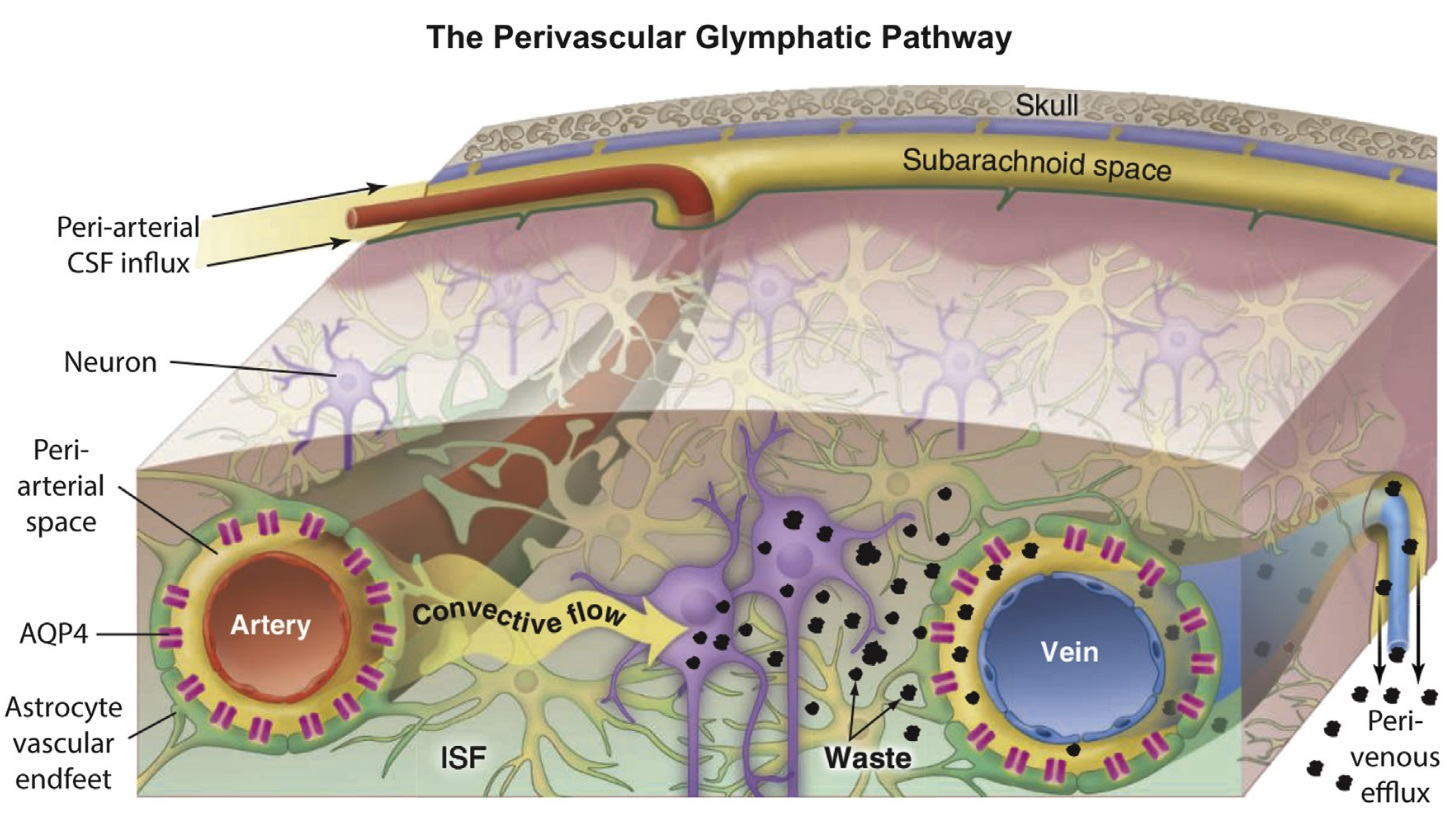
\includegraphics[scale = .6]{Figures/Iliff_2017_GlymphaticSystem.jpg}
    \caption{Diagram of the glymphatic system \citep{Nedergaard2013}}
  \label{fig:glym}
\end{figure}

One of the most important findings about the glymphatic system is its potential mechanistic link with AD. Along with other metabolites, glymphatic activity increases the clearance of both A$\beta$ and tau \citep{Iliff2012, Iliff2014, Xie}. Furthermore, this link is bidirectional, in the TgArcSwe mouse model of AD AQP4 polarization to endfeet was suppressed, and a similar effect has been shown to occur with age \citep{Yang2013, Kress2014, Zeppenfeld2017}. In another mouse model, AD APP/PS1, it was shown that glymphatic failures preceeds deposits of A$\beta$, but also that A$\beta$ exacerbates the issue by further inhibiting flow \citep{Peng2016}.

%Traumatic brain injury reduces glymphatic clearance by around 60$\%$. Impairing glymphatic system promotes tau pathology following TBI. AQP4 knockouts increase neurodegeneration and inflammation following TBI. Reactive astrocytes have reduced polarity of AQP4 disrupting perivascular structure. \citep{Iliff2014}

%%%%%%%%%%%%%%%%%%%%%%%%%%%%%%%%%%%%%%%%%%%%%%%%%%%%%%%%%%%%%%%%%%%%%%%%%%%%%%%%%%%%
%%%%%%%%%%%%%%%%%%%%%%%%%%%%%%%%%%%%%%%%%%%%%%%%%%%%%%%%%%%%%%%%%%%%%%%%%%%%%%%%%%%%
\section*{Aging and Alzheimer's Disease}
%%%%%%%%%%%%%%%%%%%%%%%%%%%%%%%%%%%%%%%%%%%%%%%%%%%%%%%%%%%%%%%%%%%%%%%%%%%%%%%%%%%%
%%%%%%%%%%%%%%%%%%%%%%%%%%%%%%%%%%%%%%%%%%%%%%%%%%%%%%%%%%%%%%%%%%%%%%%%%%%%%%%%%%%%
\subsection*{Amyloid-$\beta$ and Tau}
Since Alzheimer's dementia was first described by Alois Alzheimer as presenile and senile dementia, it has been diagnosed by the presence of senile plaques and neurofibrillary tangles, which were later discovered to be protein aggregates of amyloid-$\beta$ (A$\beta$) and phosphorylated tau \citep{Berrios1990}. Both A$\beta$ and tau are proteins associated with normal brain activity, but the accumulation of the protein aggregates are toxic.

A$\beta$ is formed when amyloid precursor protein (APP) is embedded in a cell's membrane and subsequently cleaved by $\beta$- and $\gamma$- secretases\citep{Vassar1999}. The protein is found in various cells of the body, and is particularly concentrated in the synapses of neurons \citep{Priller2006a}. Although the native role of APP has remained elusive, there are suggestions that it may be necessary for neuronal migration, the correct functioning of synapses, and cell adhesion \citep{Mattson1997,Young-Pearse2007,Priller2006a}. 

%**
Tau, the protein responsible for the formation of tangles is a microtubule associated protein, which stabilizes the formation microtubule \citep{Wang2016}. However, when it becomes phosphorylated, it is no longer able to stabilizes the microtubules. It can become misfolded making it insoluble, and form aggregate, or tangles \citep{Iqbal2016}. These tangles are especially pathogenic because they are able to spread to nearby neurons, and like a prion, cause more tangles to form.

%**
\subsection*{Sleep and aging}
Older adults encounter problems with sleep which worsen age; for instance, it takes longer to fall asleep, sleep decreases in duration, awakenings occur more frequently throughout the night and more readily in response to disturbances, and most of sleep is spent in NREM1 $\&$ 2 (rather than NREM3 or REM). Somewhat unsurprisingly, older populations report more daytime sleepiness and engage in unplanned naps. Both the power and quantity of SWs as well as spindles are reduced with age.\citep{Mander2017} Furthermore, the typical coupling of spindles with SWs that is correlated with memory consolidation is reduced in older adults \citep{Helfrich2018}. Time spent awake, increases homeostatic sleep pressure, and if sleep deprivation is sufficiently prolonged SW activity increases and is correlated with lapses in performance on cognitive tasks humans.\citep{Rodriguez2016,Watson2016,Nir2017}. Amyloid-$\beta$ accumulates with time spent awake \citep{Bateman2006,Kang2009, Xie Mander2015}%[and tau?]

%%%%%%%%%%%%%%%%%%%%%%%%%%%%%%%%%%%%%%%%%%%%%%%%%%%%%%%%%%%%%%%%%%%%%%%%%%%%%%%%%%%%
%%%%%%%%%%%%%%%%%%%%%%%%%%%%%%%%%%%%%%%%%%%%%%%%%%%%%%%%%%%%%%%%%%%%%%%%%%%%%%%%%%%%
%Trash
%%%%%%%%%%%%%%%%%%%%%%%%%%%%%%%%%%%%%%%%%%%%%%%%%%%%%%%%%%%%%%%%%%%%%%%%%%%%%%%%%%%%
%%%%%%%%%%%%%%%%%%%%%%%%%%%%%%%%%%%%%%%%%%%%%%%%%%%%%%%%%%%%%%%%%%%%%%%%%%%%%%%%%%%%
%Tonic activation of CMT causes NREM-wake transitions, while burst stimulation firing resembles up states in cingulate and promotes SW actiivty. Up-states are preceeded by firing in centromedial thalamus neurons. \citep{Gent2018}
%Ventromedial thalamic nucleus activity is low during NREM, increases during NREM-wake transition and stimulation induces a NREM-wake transition, caused activity in anesthesized animals, but did not disrupt REM sleep. \citep{Honjoh2018}

%% Staging
% These scoring criteria (with some slight modifications for other animals), have provided the standard framework to further study sleep. For instance, these are the stages used by clinicians to diagnose sleep disorders, and to study sleep induced biochemical changes. Likewise, this system has been a powerful influence on our understanding of sleep. While this standardization provides a common language for sleep necessary for building knowledge in this domain, it also creates a certain rigidity. The scoring criteria has remained essentially unchanged until 2007, when the AASM consolidated NREM3 and NREM4 into NREM3. While useful, a rigid framework may also impose artificial constraints scientific questions.
%%
%% Waves
%The body is composed of many cells of various types communicating with others at various distances and timescales. Most cells communicate by releasing signaling molecules. These signals can be passed almost immediately to a cell’s direct neighbors if there are gap junctions linking the cells; otherwise, the signal must diffuse through the extra-cellular space to reach its destination. A random walk through the tightly packed extracellular space means that the probability of a signal reaching a particular cell within some period of time falls off very quickly with distance. This problem is mitigated by the many vessels in the body providing less hindered directed channels of flow, and often propulsion to increase the speed. Although the neuron is subject to the same constraints, but it is exceptional in its ability to communicate quickly and at long distances because of a few remarkable adaptations. First, neurons leverage fast ionic conductivity by manipulating electrostatic and concentration gradients with dynamically tuned micro-fluidics. Second, some neurons have highly elongated processes which can grow to very long distances. These are far from the only remarkable features of neurons, but together, these adaptations effectively allow neurons to communicate with very distant cells as if they were next-door neighbors. While the evolutionary importance of features can hardly be overstated, the majority of neurons communicate over relatively short distances.
%The brain is a physical system basically composed of cells that can integrate many inputs, and over some threshold, project signals as input to other cells. However, inputs can vary widely in function, some on short timescales by raising or lowering the cells membrane potential, or others in some way re-tuning the cell - e.g. RNA transcription. Furthermore, these neurons can be arranged to create circuits, which are organized together perform complex computations.
%This ionic conduction also enables scientists to monitor the activity of neurons with electrophysiology. Population activity 
%These neurons can be quickly and precisely altered by various ion channel proteins in the membrane. short to long distances  physical system composed of many cells with different conductances that can integrate many inputs, and above some input threshold, project signals as input to other cells, and these cells 
%With extracellular electrophysiology, even for micro-electrodes capable of single unit recordings, it is difficult to determine the type of input or output.  of groups of neurons synchronizes to form oscillatory rhythms. 
%So, unless there is another source of the EEG signal besides neuronal activity, a global SW would entail that many widely distributed neurons are simultaneously activated and deactivated. Probably the easiest way to coordinate this would be for a single generator to send a signal to every area; however, conduction speed would lead to imprecise delivery times, unless this generator were located precisely the same distance from each region or somehow tuned to compensate for conduction.
%In contrast, a perfectly local signal would be one that is isolated to a single area, and not spread to other areas. In a less strict interpretation, a local signal might be one that occurs in one location, but could be sent to another location. This is unlikely because nearby areas are more highly connected.%Perhaps particular waveforms are emerge out of reaction diffusion stability. The detection of travelling waves could be used to infer effective connectivity. If this is the case, mapping the spatiotemporal repertoire of these waveforms may suggest its principal source and sinks, functional/computational role, facilitate a predictive model, etc. 
%So it is much more likely that there is a spread of activity into surrounding areas in addition to saltatory transmissions of activity to more remote areas, which in turn spread locally.
%The brain has very neurotransmitters, some with very exotic downstream effects, but on short-timescales most of them impart a transient change in ionic permeability increasing (excitatory) or decreases (inhibitory) voltage, and likewise firing probability. Furthermore, the connectivity of the neurons imparts a structure over which the excitatory and inhibitory signals can propagate. The dynamics of this system have been characterized as a reaction-diffusion system, which was famously introduced and analyzed by Alan Turing \citep{Turing1952}
%One of the most interesting features, of such systems are their extensive repertoire of spatiotemporal dynamics. Even simple systems can be tuned to reproduce patterns like leopard spots, and over time these patterns evolve as traveling waves of patterns

%% SW
% The up and down state can be partially explained by afterhyperpolarizations produced by Ca$^{2+}$ mediated increases in K$^+$ conductance in soma [47,48].
% Bereitschatfspotential, or readiness potentials, associated with surprise or initiation of movement cause synchronized afterhyperpolarizations which can produce a SW [50,51].
% Synchronized bursting pyramidal cells during NREM produce large dipole from positive infragranular and negative supragranular layers [48, 54-56].
% interneurons and thalamocortical inputs to pyramidal cells are active during down states [52,53,57,58]. 
% Cyclic nucleotide-gated hyperpolarization deinactivated (I$_h$) and low-voltage hyperpolarization-induced T-type Ca$^{2+}$ channels (I$_T$) create intrinsic cell resonance and produce oscillations of membrane potential which are unrelated to synaptic events [39]. In pyramidal cells this may produce theta rhythms [41-44], while in interneurons this may produce gamma rhythms [45,46]
% \citep{Buzsaki2012}
% Slow-waves are believed to emerge from the interactions between the cortex and the thalamus.
% Low-voltage gated T-type Ca$^{2+}$ channels cause low-threshold spike (LTS) Ca$^{2+}$ spikes causing rhythmic bursting with intraspike frequencies between 100-500Hz. 
% In contrast, alpha and theta waves are thought to be driven by both high-threshold spikes produced by both low T-type and high L-type voltage-gated Ca$^{2+}$ channels causing lower frequency bursting between 50-70 Hz.
% The source of EEG are supragranular cortical cells, but these involve thalamocortical interaction.
% While, \textit{in vivo} thalamic neurons produce only short delta oscillations, in decorticated animals, these oscillations are sustained (consistent with cortical disfacilitation during down states) [21-24].
% Unlike cortex, delta oscillations in the thalamic neuron rely on LTS bursts [4,20,25]
% "conclusively demonstrated in anesthetized and sleeping animals that SW EEG requires thalamic participation" [30, 37], but in isolation distinct mechanisms produce SW.
% SW are significantly reduced if synaptic transmission is blocked [21,22,38]
% TC neurons generated SW with K$^+$ leak, I$_T$, I$_{CAN}$, and I$_h$ [9, 11, 17, 39]. NRT neurons are similar, but also require Na$^2+$ and Ca$2+$ activated K$^+$ currents [34]. Furthermore, these can be transformed into delta rhythms with by changing the membrane potential via I$_T$ [11,17,39]. Notably, delta oscillations can occur during SW [5,6,9,34].
% \citep{Crunelli2018} 

%%Memory
%Nevertheless, it seems that during down states CA3 and CA1 are able to generate gamma bursts and ripples.
%Recurrent local circuits of deep cortical layers may produce SW and synchronize large swaths of cortex via long-range cortical connections in superficial layers. They hypothesize that an excitatory front of the SW spreads from cortex to entorhinal cortex to hippocampus, which is supported by consistent delay times. An important physiological role of SW is to coordinate locally emerging patterns. Integration and Segregation of Activity in Entorhinal-Hippocampal Subregions by Neocortical Slow Oscillations\cite{Isomura2006}
%Network homeostasis and State Dynamics of Neocortical Sleep \citep{Watson2016}
%IEDs hijack ripple band in rodent epilepsy models and associated with reduced memory consolidation. These IEDs induce SWs. \citep{Gelinas2016}

%CA
%Astrocyctes induce neuronal hyperpolarization via decreasing K$^+$ associated with Ca$2+$ signaling which increases signal to noise ratio of synaptic transmission. \citep{Wang2012}
% Reduced spontaneous as well as stimulation and agonist induced local somatic and process transients in addition to global, synchronized Ca$2+$ transients. Signaling in astrocytes is reduced temporally before neurons and at lower doses. While astrocytic Ca$2+$ signaling is critically dependent on IP3R2, it was only slightly reduced when neuronal signalling was blocked. \citep{Thrane2012}
%Astrocytic phagocytosis increases with sleep deprivation.

%% General
%The consequences of sleep deprivation are a growing list including loss of sex drive, elevated blood pressure, weakened immunity, cognitive impairment, and increased risk for a wide range of diseases. So while unconsciousness is the most obvious feature of sleep, it is just a side-effect of this profound state change which facilitates critical homeostatic processes throughout the body - especially in the brain. Around sleep onset, movement and sensory stimulation decrease, along with the demand for oxygen by the tissues serving these functions, thus permitting respiration to slow and the heart relax. As the brain falls deeper into sleep, the concentration of neuromodulatory transmitters, like norepinephrine and serotonin, decrease, and neuronal activity increasingly alternates between active and inactive firing states modulated by ~1 Hz waveforms called slow waves (SW). In parallel, astrocytes reduce their rate of anaerobic glycolysis, seek out synapses to phagocytose, and alter ionic composition of extracellular cerebrospinal fluid (CSF) in addition to permitting greater flow of CSF into/out of the brain. Importantly, these sleep processes and others have strong connections to cognition, aging, and disease, but some of these findings are inadequately studied in humans mostly limited by suitable methods that also meet the paramount ethical considerations for studying human subjects.
%Like the rest of nature, the life of an organism consists of persistent cycles interweaving with one another to support the whole.
%The development of the brain is a story of neurons and glia eventually emerging together as daughters of the gastrula's neural crest cells. These cells organize themselves into a complex pattern harmonizing with the parallel development of the vascular system and overcoming space constraints of the skull by folding as it continues to expand. Of course, this development does not stop after birth, but continues, albeit in a different way, as the organism adapts an environment and body in constant change.
%Importantly, during sleep as well as wake, neurons do not operate in isolation, but are supported by the entire body, and most intimately by its direct relatives the glia. Yet despite this critical dependence, studies of the human brain have a tendency to fixate on neural factors.
% Sleep is a great model to study interactions between brain systems because the activities of both neurons and glia change so markedly between these two states. Furthermore, sleep dysfunction is a risk factor for many diseases, especially of the brain. 
% I hope to identify mechanisms of interaction between systems supporting brain function by developing approaches that enhance existing imaging techniques through the integration of multiple data modalities.
% Longterm, homeostatic importance of sleep, and interaction of various systems to support the brain.
% I think the neuroscience of sleep is intimately related to the work of non-neuronal cells forming a robust infrastructure that supports the strenuous activity and intricate, but fragile structure of the nervous system.
%Later Antoine Louveau and Jonathan Kipnis showed evidence of a more traditional lymphatic vessel incorporated in the brain’s dura, which has been termed cerebral lymphatic vessels.

%Many synpatic sleep-need-index phosphoproteins (SNIPPS) which phosphorylate with wake and dephosphorylated during sleep. A phosphorylating protein called SIK3 drove sleep need by phosphylating SNIPPs. \citep{Wang2018}

%%% Local Variables: ***
%%% mode: latex ***
%%% TeX-master: "thesis.tex" ***
%%% End: ***
